
\chapter{Conclusion and Perspectives}\label{section:generalconclusion}
\addcontentsline{toc}{chapter}{Conclusion}


The primary aim of this work was to develop a simulation framework capable of assessing the quality of breast compression in function of the paddle design, compression force intensity or breast positioning. The image quality and the average glandular dose as well as the patient comfort have to be considered then comparing different compression strategies.

 Monte-Carlo based simulation able to compute the X-ray propagation trough matter are well known and largely accepted on the field. Such software was used to mimic a mammography exam and thus to assess the image quality depending on the compressed breast thickness. The average glandular dose was computed using the method proposed by \citep{dance_additional_2000}. The method was build based on a very simplistic template and requires only the knowledge of the compressed breast thickness and breast glandularity. 
 
 To assess the tissues deformation depending on the paddle design or the applied force a biomechanical model is used. The latter allows to estimates the outer breast shape after compression but also the physical patient comfort associated to the internal strain/stress intensity and distribution.
 
 In this chapter, the main results and conclusions on the implemented applications are recalled. The possible improvements for a large prospect of applications are discussed. 
 \clearpage
 \section{Biomechanical breast model }
  Before modeling the mammography breast compression, the model fidelity to the real tissues deformation had to be assessed. In this  scope, subject specific data describing the in-vivo breast mechanics were needed. The MRI is the sole imaging modality allowing to extract the hole 3D breast geometry and the corresponding internal structures distribution.  Therefore, MR images of two volunteers in three body positions, prone, supine and supine tilted were acquired and used in this study. The boundary conditions describing breast deformation under gravity loading are easy to reproduce in a simulation framework. Thus the acquired data made possible the biomechanical model calibration and evaluation.
  
 The MRI volume of breast in the supine position was used to build the finite element mesh. Then, combined with the MRI breast volume from the prone body position, it was used to estimate the subject specific constitutive parameters and the corresponding the stress-free geometry. 
 
 The first simulations showed the importance of considering the sliding boundary conditions at the juncture surface between  the muscle and the breast. The deformation due to the tissues elasticity only, was not enough to reflect the geometrical changes between the supine and prone breast configurations. Therefore the breast tissues were allowed to slide over the muscle surface. Additional boundary conditions were considered by modeling the breast suspensory ligaments and fascial system. Including stiffer structure into the finite element model improved solution convergence capabilities. This new structures allowed to estimate the breast deformations for a larger range of constitutive parameters of soft tissues. Consequently, the result of the model optimization process was improved.   
 
 According to the literature, a well defined breast model have to consider in-vivo measured constitutive parameters. To this end, the tissues Yound's modulus giving the best fit between the simulated and measured breast geometries were computed. The optimal estimates, assuming Neo-Hookean materials models, were given by $\lambda_{breast}^r=0.3\ kPa$, $\lambda_{breast}^l=0.2\ kPa$, $\lambda_{skin}=4\ kPa$, $\lambda_{fascia}=120\ kPa$. The obtained mechanical properties are comparable with the ones proposed in the literature then considering only the breast models with similar simulation frameworks \cite{rajagopal_modelling_2007, gamage_modelling_2012, griesenauer_breast_2017}. These results allowed to compute the breast geometry in supine and prone configuration within an error of $1.70\ mm$ and $2.17\ mm$ respectively. 
 
The model fidelity to the global breast deformation was evaluated using the supine tilted position. The Hausdorff distance between the breast skin surface extracted from the MRI volume and the simulated skin surface was equal to $6.14 \ mm$. The larger error ($\sim 26.03 \ mm$) is obtained on the left breast where the tissues lateral displacement is overestimated. These results may be improved by developing a more complex breast support matrix or region dependent stiffness for some tissues as the skin or the fascial system. Adding stiffer materials in the strategically localized areas on the contact surface may limit the fascia deformations under large stress ranges. Therefore, the breast tissues sliding in supine tilted configuration may be reduced. 

Despite providing good results in a multi-loading gravity framework, the optimized breast model turn out to be less efficient in simulating the breast tissues compression. The maximal force needed to simulate the breast flattening was estimated relatively small then compared to the mean recommended force for a mammography exam (10 N vs 100 N). The low value of the compression force is caused by the tissues abnormal softening under large stress rates. Tissues relaxation from a given stress threshold is a well known phenomenon then using Neo-Hookean materials . This issue was overcome by replacing the Neo-Hookean model by a Gent model for all involved hyperelastic tissues.

 The advantage of using the Gent strain energy function is its similarity with the Neo-Hookean function. The stress-strain relation remains the same for both models bellow a strain threshold defined by the $J_m$ parameter. Beyond the respective threshold the Gent materials model is stiffening exponentially resulting in an asymptotic behavior . These properties allowed to change the tissues mechanical response only for large strain rates, as during the breast compression. And on the other hand, allowed to preserve the same mechanical response for relatively small strains as induced by gravity loading simulations.

Using a Gent material model improved the tissues mechanical response then compressed between the paddle and the image receptor. A compression force of $22 \ N$ was estimated for the first volunteer which fit well with the corresponding clinical data ($21.9 \ N$). Then looking back to gravity loading simulations, introducing a Gent tissues model must not impact the breast deformation obtained in prone and supine configurations. However, for the supine tilted configuration, large deformations were observed at the fascia and skin surfaces. Figure \ref{fig:strain_range_neo} shows the strain rates in supine, prone and supine tilted configurations obtained with Neo-Hookean material models. The strain rates over the skin and fascia surfaces in supine tilted configuration were twice larger than ones observed in supine and prone breast configurations. Therefore, considering the Gent model in the multi-loading gravity simulations may reduce the fascia and skin deformations under large stresses. 


\begin{figure}[!h]
\centering
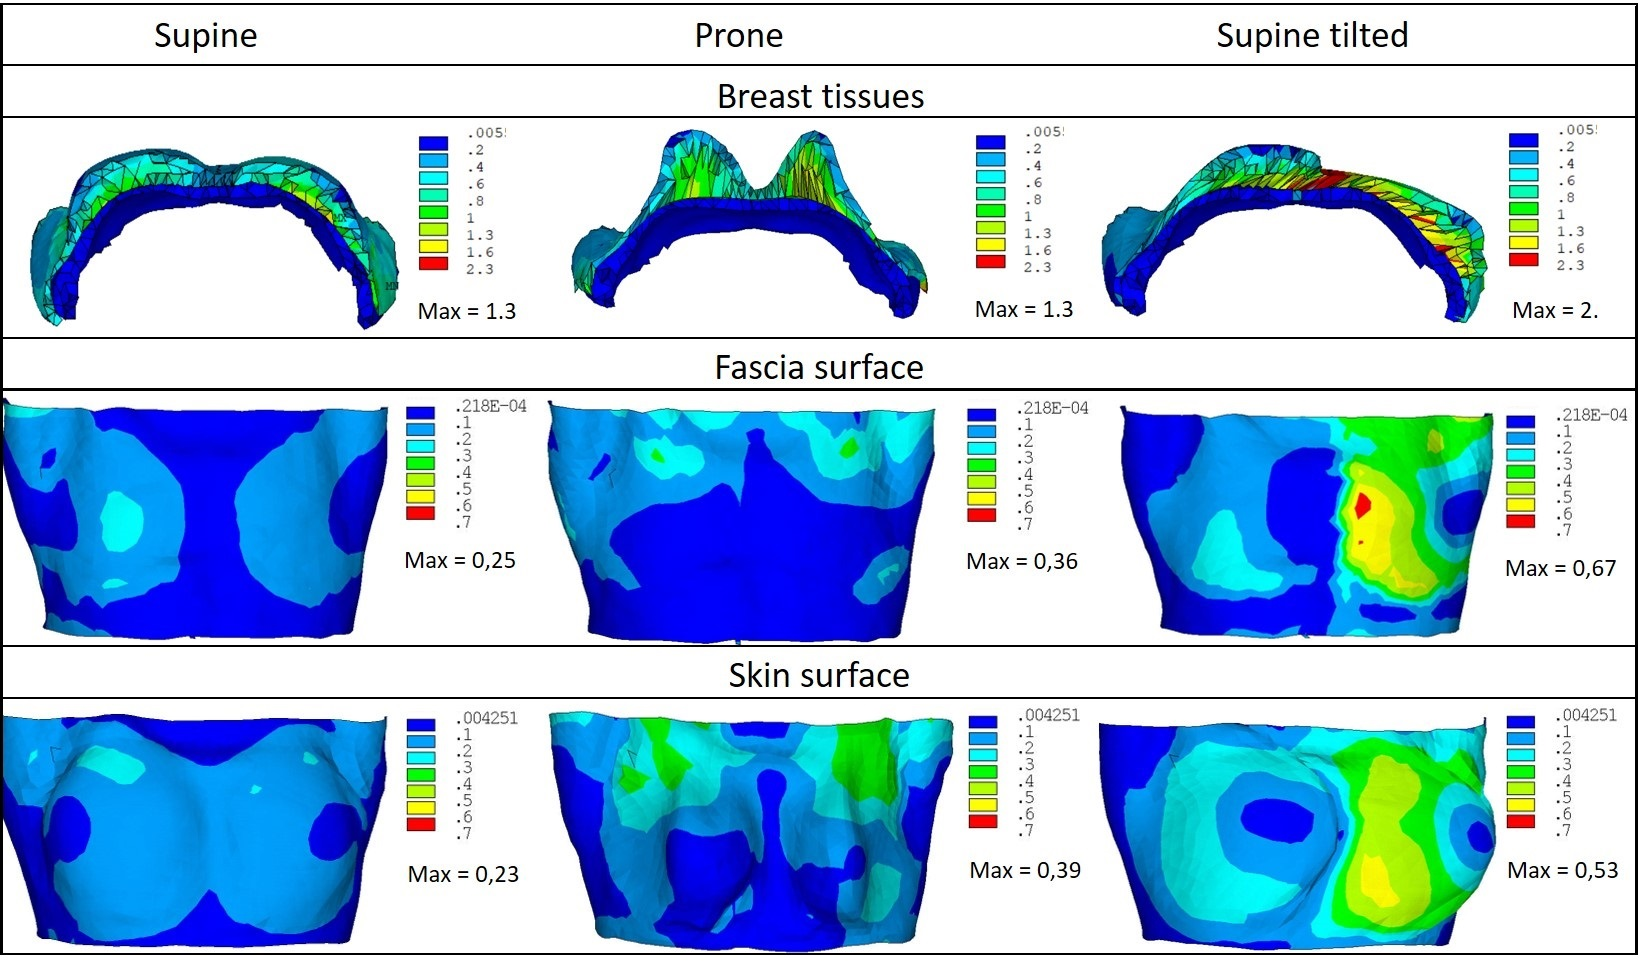
\includegraphics[width=\textwidth,keepaspectratio]{figures/strain_range_neo.jpg} 
\caption{Strain range distribution when using a Neo-Hookean material model. }\label{fig:strain_range_neo}
\end{figure}
 

\begin{figure}[!h]
\centering
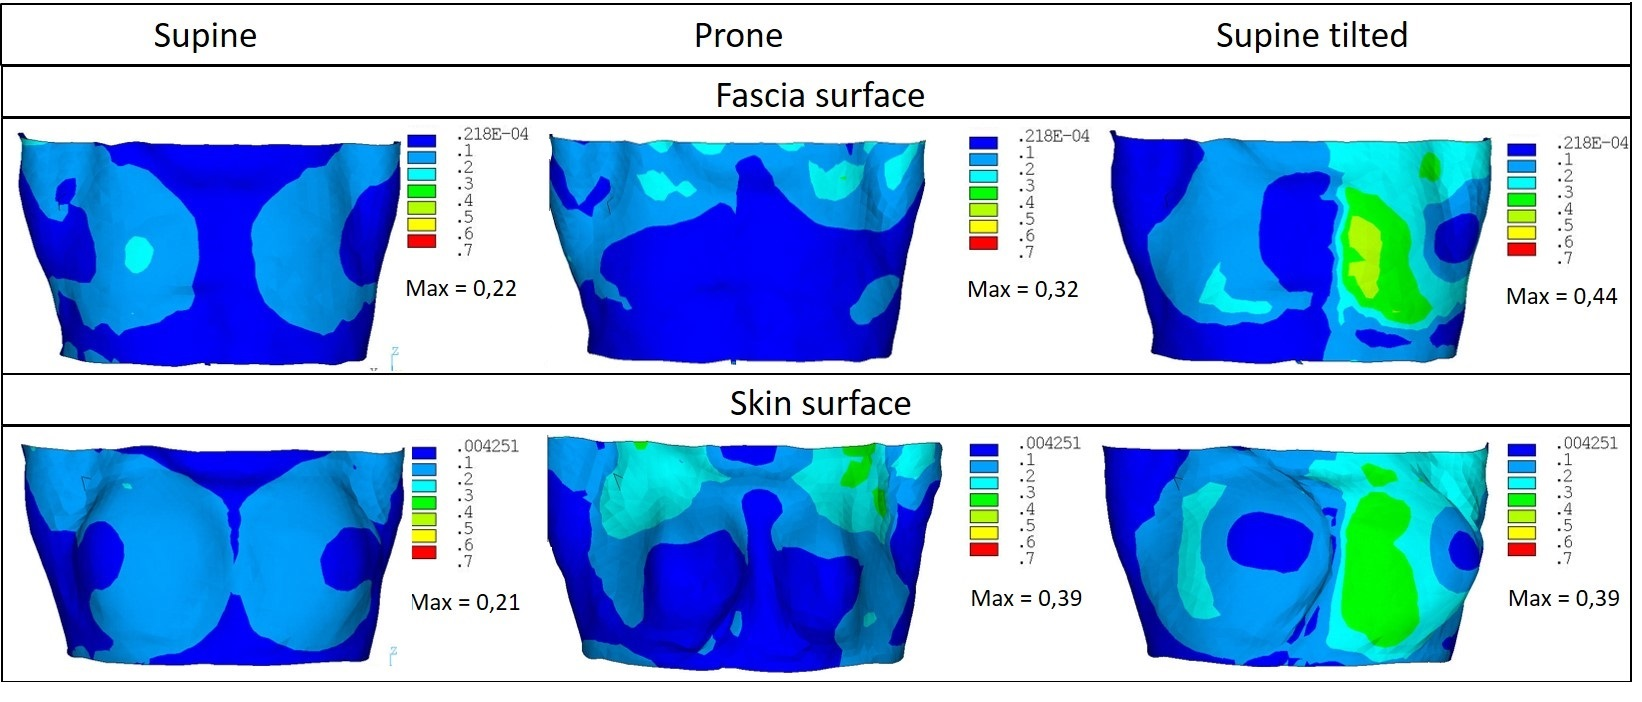
\includegraphics[width=\textwidth,keepaspectratio]{figures/strain_range_gent.jpg} 
\caption{Strain range distribution when using a Gent material model. }\label{fig:strain_range_gent}
\end{figure}

Preliminary simulations were performed using Gent material models. The $J_m$ parameter was quipped to the same value as estimated during compression simulations ($J_m = 2$). However, in Section \ref{subsection:breastpositioning} we have seen that, the compression force is highly dependent on the breast positioning with respect to the chest wall. Therefore, for an accurate estimation of the $J_m$  parameter, more data is needed concerning the breast position during compression. 


Figure \ref{fig:strain_range_gent} shows the corresponding strain rages distribution over the skin and fascia surfaces.  The maximal strain does not change significantly in supine and prone configurations ($\sim 10\%$). On the other hand, an important change was observed over the left breast in supine tilted configuration. The maximal strain rage decreased by about $30\%$ over the fascia surface and by about $26 \ \%$ over the skin surface. As previously described, these tissues provide the breast support, accordingly,  the lateral displacement of the left breast was reduced.

 The estimates of the breast geometry in the three configurations computed using the Gent material models are presented in Figure \ref{fig:modelevaluation_gent}. One may see that, the breast deformations in supine and prone configurations remain on the same rage of precision. The Hausdorff distance being increased by only $0.46 \ mm$ and $0.6\ mm$ respectively (maximal distance by $0.17$ and $0.93 \ mm$ respectively). Contrariwise, the sliding of the left breast was significantly reduced. Even if the Hausdorff distance was reduced by only $1 \ mm $ ($5.15 \ mm$ with Gent models versus $6.14 \ $ with Neo-Hookean models), an significant decrease of $10 \ mm$ in maximal distance  was observed. Moreover, smaller deformations implies also better solution convergence. 
   

\begin{figure}[!h]
\centering
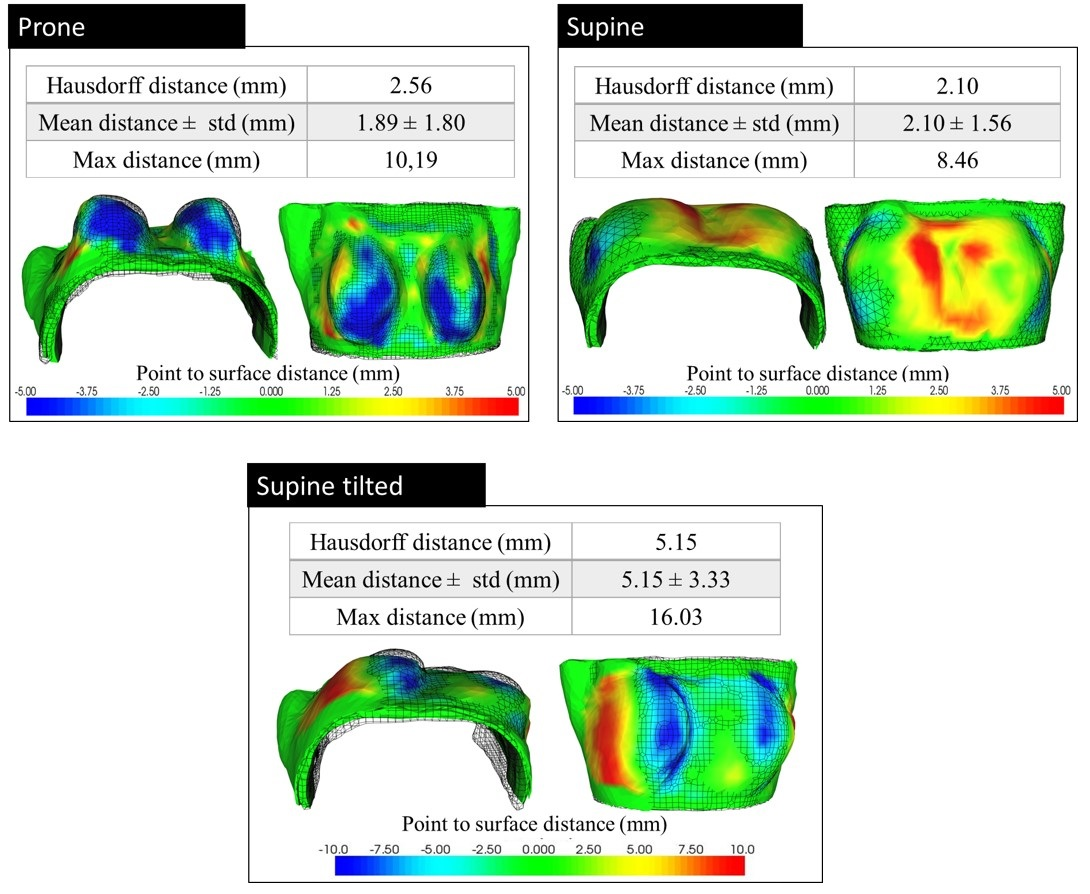
\includegraphics[width=\textwidth,keepaspectratio]{figures/modelevaluation_gent.jpg} 
\caption{Difference between estimated and measured data, in supine, prone and supine tilted configurations obtained with a Gent material model. }\label{fig:modelevaluation_gent}
\end{figure}

Using the Gent model improved the overall performance of the breast biomechanical model. However, a more accurate estimation of the $J_m$ parameter is required. We assumed a constant value for all involved hyperelastic material models, yet their mechanical response under large stresses are different. A variable $J_m$ parameter within tissues types may improve the model accuracy.  On the other hand, it also implies an optimization process with more constitutive parameters. An optimization process with a higher number of variables is also more expensive in terms of data and time resources. 

In conclusion, the proposed biomechanical model was able to estimate the breast deformation for both loading frameworks, multi-loading gravity or compression. However it was calibrated for only one subject geometry and mechanical properties. It would be interesting to evaluate the model accuracy on at least two more subjects with different breast morphology and mechanical properties. The model calibration on a larger population will improve its flexibility for further studies on breast compression techniques.   

\section{Breast compression and patient comfort}
The developed biomechanical breast model together with the image simulation framework were used to assess the clinical compression quality then using different compression strategies.

Flex and rigid paddle compression were compared for two breast volumes. The results showed that, using the flex paddle may improve the patient comfort without affecting the image quality and the delivered average glandular dose. Moreover, despite a breast thickness varying linearly from chest wall to nipple the image quality seems to be preserved or improved compared to the image quality obtained with a rigid compression paddle. The improved image quality for the flex paddle could be explained by a better overall breast compression. The paddle tilt allows a better compression of the tissues closer to the nipple and in the same time relaxing the tissues closet to the chest wall. In the same time, the paddle tilt is suspected to facilitate the tissues displacement toward the chest wall.  The tissues accumulation on the retromammary space may hide clinical relevant information ans thus increase the false negatives rates. 

However, not all mechanical properties of the standard rigid and flex paddles were considered in the previous study. The paddle deflection due to the material elastic properties should be included for a better estimation of the patient comfort and image quality. Therefore, to study the impact of breast positioning on the compression mechanics, a paddle model considering the material elasticity was used. The result showed that the patient comfort can be improved by positioning the paddles farther from the pectoral muscle. For an equivalent breast thickness, the compression force decreased from 158 N to 59 N for a difference of 15 mm in the distance from chest wall to the paddle. On the other hand, clinical guidelines request to place the paddle as close as possible to the chest wall. Therefore, the technologist have to find a compromise between the exam quality and the patient comfort. 

The two preliminary applications have shown the feasibility  to asses the clinical compression quality by using simulation frameworks. The developed tools may be used to perform wider studies comparing the already know breast compression paddles. But also to provide a first estimation of the performance of a new, not yet implemented, paddle design. Simulation based studies are less expensive in time and materials that the usual clinical studies, therefore they may be used to discharge the more deficient designs.

\cleardoublepage



\chapter*{Key contributions}\label{section:keycontributions}
\addcontentsline{toc}{chapter}{Key contributions}
\markboth{\textsc{Key contributions}}{}

The key contributions concerning the finite element breast modeling are the following:

\begin{itemize}
\item We introduced new boundary conditions which reflect the motion of the breast over the thoracic cage.  They included sliding contact surface based on Coulombs friction law combined with stiff support structures. To our knowledge,  the breast support matrix was considered for the first time into the finite element model. The generic model include suspensory ligaments together with the fascial system, and was built based on their anatomical description .   

\item The iterative algorithms allowing to estimate the breast stress-free  geometry are generally using only one configuration (supine or prone breast configuration). In this work we proposed an optimization algorithm which estimate the breast stress-free geometry starting from supine configuration and then iteratively correct it based on the prone configuration. 

\item  We disposed of an exceptional data set of breast MR images in three different body positions. Therefore, the biomechanical breast model was first calibrated using prone and supine configrations. Then, its mechanical response was evaluated on the third breast configuration (supine tilted). Because of a lack of reliable data, non of previous biomechanical breast models was evaluates in such board range of deformations.  

\item We evaluated the capability of the proposed biomechanical beast model to reproduce the breast compression mechanics as described by several clinical studies.  The simulations results were then compared with the data acquired form the volunteers last mammogram. This analysis allowed us to point out the limitations of the Neo-Hookean strain energy function then modeling such large deformations.  Accordingly, a new material contitutive model defined by the Gent strain energy function was proposed.


\item We developed a simulation framework allowing to quantify the breast compression quality in therms of image quality, average glandular dose and patient comfort. Due to its modularity, the framework supports different paddle designs and different breasts geometry and compositions. 
\end{itemize}

Using previously described tools, two studies assesing the breast compression quality were performed.

\begin{itemize}
\item The difference of the compression quality in therms of patient comfort, image quality and average glandular dose between a standard rigid and flex paddles was quantified.
\item The impact of breast positioning on the compression mechanics and patient comfort was analyzed. 
\end{itemize}
A list of publications resuming the results of this work is provided below.
\cleardoublepage
 
\chapter*{Publications}\label{section:publications}
\addcontentsline{toc}{chapter}{Publications}
\markboth{\textsc{Publications}}{}

\begin{description}

\item  Mîra, A., Payan, Y., Carton, A. K., de Carvalho, P. M., Li, Z., Devauges, V., \& Muller, S. (2018, March). Simulation of breast compression using a new biomechanical model. \textit {In Medical Imaging 2018:Physics of Medical Imaging} (Vol. 10573, p. 105735A). International Society for Optics and Photonics. \\

\item  Mîra A., Carton A.K., Muller S. \& Payan Y. (2018). Breast biomechanical modeling for compression optimization in digital breast tomosynthesis. \textit{Computer Methods in Biomechanics and Biomedical Engineering}, Lecture Notes in Bioengineering, A. Gefen and D. Weihs editors, pp. 29-35, DOI $10.1007/978-3-319-59764-5\_4$ \\

\item  Mîra A., Carton A.K., Muller S. \& Payan Y. (2016). Breast biomechanical modeling for compression optimization in digital breast tomosynthesis. \textit{Proceedings of the 22nd Congress of the European Society of Biomechanics (ESB2016)}
\end{description}

\cleardoublepage